%---------------------------------------------------------
\begin{frame}{Divert FAIR data principles towards processes}
\begin{columns}[t]
  \begin{column}{.25\textwidth}
      \begin{center}
      
\includegraphics[height=1.5cm]{01_introduction/images/logo-FAIR-F.png}\\Third party tools used = ref. in their field\\.\\Easy to find analysis protocol (Github pages)
      \end{center}
  \end{column}
  \begin{column}{.25\textwidth}
      \begin{center}
      
\includegraphics[height=1.5cm]{01_introduction/images/logo-FAIR-A.png}\\Available codes (Github, dockerhub)\\.\\Third party open source tools
      \end{center}
  \end{column}
  \begin{column}{.25\textwidth}
     \begin{center}
     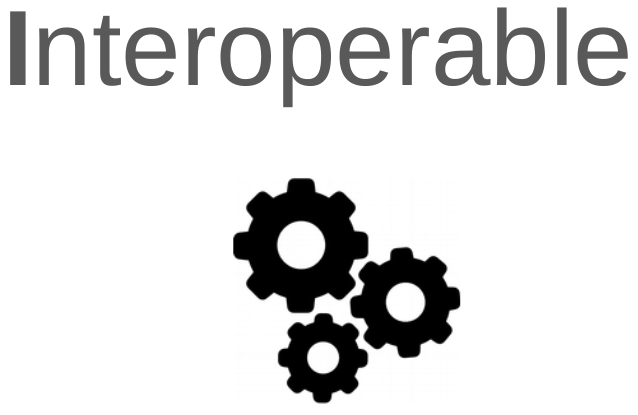
\includegraphics[height=1.5cm]{01_introduction/images/logo-FAIR-I.png}\\Cooperation of tools (snakemake, docker) as well as locally than on servers (cloud or cluster)
     \end{center}
  \end{column}
  \begin{column}{.25\textwidth}
     \begin{center}
     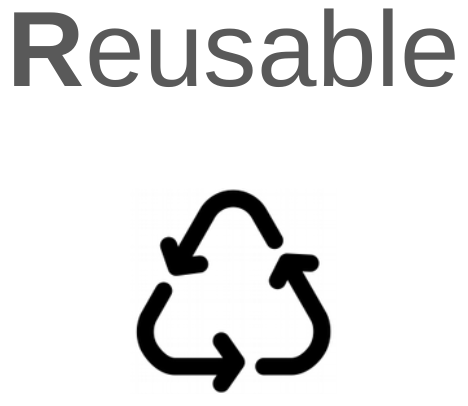
\includegraphics[height=1.5cm]{01_introduction/images/logo-FAIR-R.png}\\Protocol replayable (snakemake) identically (Rshiny) in a virtual environment (docker)
     \end{center}
  \end{column}
\end{columns}
\end{frame}
%---------------------------------------------------------
\begin{frame}{Promote learning}  
  \begin{columns}
    \begin{column}{.3\textwidth}
     
\includegraphics[height=2cm]{shared/FAIR_logo.png}
     \begin{block}{Our objective}
       \begin{center}
       FAIR raw data\\
       +\\
       FAIR scripts\\
       =\\
       FAIR processed data
       \end{center}
     \end{block}
    \end{column}
    \begin{column}{.55\textwidth}
    \begin{block}{Course}
    Take your first steps with several companion tools to gain in reproducibility
    \end{block}
     \begin{block}{Example based}
       Classical RNA-seq analysis\\(finding genes with differential expression between 2 conditions)\\used as an example (not explained)
     \end{block}
    \end{column}
  \end{columns}
\end{frame}